\documentclass[a4paper]{article}

\usepackage[T2A]{fontenc}
\usepackage[utf8]{inputenc}
\usepackage[russian]{babel}


\usepackage{graphicx}
\usepackage{float}
\usepackage{mathtools}
\usepackage{wrapfig}
\usepackage{amsfonts, amssymb, amsmath, latexsym}
\usepackage{nicefrac}
\usepackage{hhline}
\usepackage{multirow}
\usepackage[colorinlistoftodos,bordercolor=orange,backgroundcolor=orange!20,linecolor=orange,textsize=scriptsize]{todonotes}
\usepackage[colorlinks=true,linkcolor=blue,citecolor=blue]{hyperref}       % hyperlinks
\usepackage{nicefrac}       % compact symbols for 1/2, etc.
\usepackage{nameref}
\usepackage{booktabs}       % professional-quality tables

\usepackage{algorithm}
\usepackage{algpseudocode}

\usepackage{xcolor, colortbl}
\usepackage{etoolbox}

% \graphicspath{ {./} }

\usepackage[verbose=true,letterpaper]{geometry}

\newgeometry{
    textheight=9in,
    textwidth=5.5in,
    top=1in,
    headheight=12pt,
    headsep=25pt,
    footskip=30pt
}

\usepackage{epigraph}

%

\usepackage{amsmath,amsfonts,amssymb,amsthm,mathtools, mathrsfs}
\newcommand{\argmin}{\mathop{\arg\!\min}}
\newcommand{\argmax}{\mathop{\arg\!\max}}

\newcommand{\Var}{\mathbb{V}}
\newcommand{\Exp}{\mathbb{E}}
\newcommand{\Cov}{\text{Cov}}
\newcommand{\makebold}[1]{\boldsymbol{#1}}
\newcommand{\mean}[1]{\overline{#1}}
\newcommand{\eps}{\varepsilon}
\renewcommand{\epsilon}{\varepsilon}

\newcommand{\partfrac}[2]{\frac{\partial #1}{\partial #2}}
\newcommand{\ttt}[1]{\texttt{#1}}
\newcommand{\term}[1]{\textbf{#1}}

\newcommand{\la}{\langle}
\newcommand{\ra}{\rangle}

\newcommand{\lp}{\left(}
\newcommand{\rp}{\right)}
\newcommand{\lf}{\left\{}
\newcommand{\rf}{\right\}}
\newcommand{\ls}{\left[}
\newcommand{\rs}{\right]}
\newcommand{\lv}{\left|}
\newcommand{\rv}{\right|}

\newcommand*{\affaddr}[1]{#1} % No op here. Customize it for different styles.
\newcommand*{\affmark}[1][*]{\textsuperscript{#1}}


\usepackage{amsthm}

\theoremstyle{definition}
\newtheorem{definition}{Определение}[section]

\newtheorem{exercise}{Задача}[section]

\newtheorem*{solution}{Решение}
\theoremstyle{remark}
\newtheorem*{remark}{Remark}

\makeatletter
\renewcommand{\l@section}{\@dottedtocline{1}{0em}{2.1em}}
\makeatother

% \setlength\epigraphwidth{.8\textwidth}
\setlength\epigraphrule{0pt}

\title{Работа 3.4.2 \\ Закон Кюри-Вейса}
\author{Шарапов Денис, Зелёный Николай, Б05-005}
\date{}

\usepackage{fancyhdr}
\pagestyle{fancy}
\fancyhf{}
\rhead{Работа 3.4.2}
\lhead{}
\cfoot{\thepage}
\usepackage{subcaption}
\usepackage[font={small}]{caption}

\begin{document}

    \maketitle
    \tableofcontents
    \newpage
    
\section{Аннотация}

\noindent\textbf{Цель работы:} изучение температурной зависимости магнитной восприимчивости ферромагнетика выше точки Кюри. \medskip
 
\noindent \textbf{В работе используются:} катушка с образцом из гадолиния, термостат, частотометр, цифровой вольтметр, $LC$-автогенератор, термопара медь-константан.

\subsection{Экспериментальная установка}

Экспериментальная установка. Схема установки для проверки Закона Кюри Вейсса показана на рис. Исследуемый ферромагнитный образец (гадолиний) расположен внутри пустотелой катушки самоиндукции, которая служит индуктивностью колебательного контура, входящего в состав $L C$ -автогенератора. Автогенератор собран на полевом транзисторе КП-103 и смонтирован в виде отдельного блока.

\begin{figure}[h!]
    \centering
    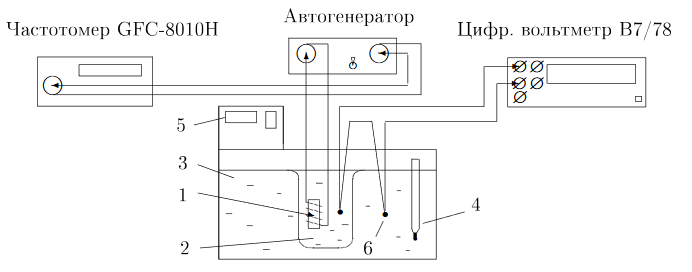
\includegraphics[width=\linewidth]{image/1.png}
    \caption{Схема установки}
\end{figure}

\noindent Гадолиний является хорошим проводником электрического тока, a paбoчая частота генератора достаточно велика $(\sim 50$ к Гц $),$ поэтому для уменьшения вихревых токов образец изготовлен из мелких кусочков размером $\sim 0,5$ мм. Катушка 1 с образцом помещена в стеклянный сосуд 2, залитый трансформаторным маслом. Масло предохраняет образец от окисления и способствует
ухудшению электрического контакта между отдельными частичками образца. Кроме того, оно улучшает тепловой контакт между образцом и термостатируемой (рабочей) жидкостью 3 в термостате. Ртутный термометр 4 используется для приближённой оценки температуры. \medskip


\noindent При изменении температуры меняется магнитная восприимчивость образца $\chi,$ а следовательно, самоиндукция катушки и период колебаний $\tau$ автогенератора. Для измерения периода используется частотомер.
Закон Кюри Вейсса справедлив, если выполнено соотношение: 
\begin{equation*}
\frac{1}{\chi} \sim\left(T-\Theta_{p}\right) \sim \frac{1}{\left(\tau^{2}-\tau_{o}^{2}\right)},
\end{equation*}

где $\tau_{o}$ --- период колебаний в отсутствие образца. \medskip

\noindent Для охлаждения образца используется холодная водопроводная вода, циркулирующая вокруг сосуда с рабочей жидкостью (дистиллированной водой); рабочая жидкость постоянно перемешивается. \medskip

\noindent Величина стабилизируемой температуры задаётся на дисплее 5 термостата. Для нагрева служит внутренний электронагреватель, не показанный на рисунке 1.

\noindent Когда температура рабочей жидкости в сосуде приближается к заданной, непрерывный режим работы нагревателя автоматически переходит в импульсный (нагреватель то включается, то выключается) - начинается процесс стабилизации температуры. \medskip

\noindent Температура исследуемого образца всегда несколько отличается от температуры дистиллированной воды в сосуде. После того как вода достигла pданной температуры, идёт медленный процесс выравнивания температур образца и воды. Разность их температур контролируется с помощью медноконстантановой термопары 6 и цифрового вольтметра. Один из спаев термопары находится в тепловом контакте с образцом, а другой погружён в воду. Концы термопары подключены к цифровому вольтметру. Рекомендуется измерять период колебаний автогенератора в тот момент, когда указанная разность температур становится $\leqslant 0,5^{\circ} \mathrm{C} .$ Чувствительность термопары $$\mathrm{K}=24 \;\;\text{град} / \mathrm{\text{мB}}.$$

\section{Результаты измерений и обработка данных}

Исследуем зависимость периода колебаний $LC$-генератора от температуры образца, отмечая период колебаний $\tau$ по частотометру, а температуру $T$ --- по показаниям дисплея и цифровому вольтметру. Результаты измерений внесём в таблицу 1.

\begin{figure}[h!]
    \centering
    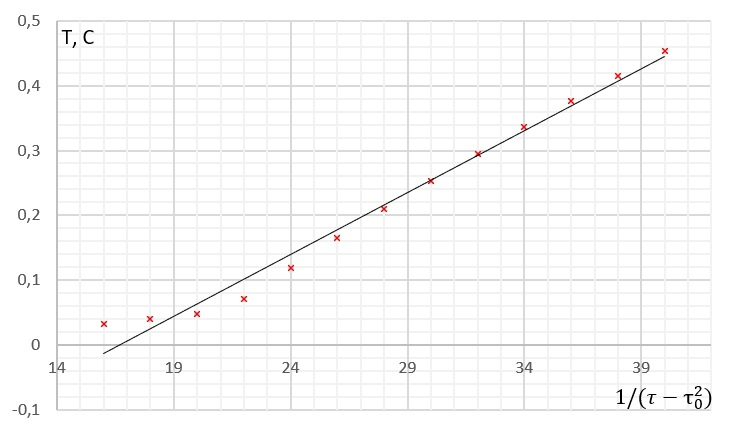
\includegraphics[width=\linewidth]{image/pic1.jpg}
    \caption{Исследование закона Кюри-Вейса}
\end{figure}

Построим график зависимости $1 / (\tau^2 - \tau_0^2)$ от $T$. Экстраполируем линейный участок зависимости, чтобы определить $\theta_p$ и $\theta_k$ для гадолиния

    $$\theta_p = 18.4 \pm  0.2^{\circ} \mathrm{C},$$
    $$\theta_k \approx 21,7 \pm 2^{\circ} \mathrm{C}.$$

\begin{table}[h!]
    \centering
    \caption{Результаты измерений}
    \begin{tabular}{|c|c|c|}
    \hline
    $T,$ $^\circ \mathrm{C}$ & $\tau$, мкс & $1/(\tau^2 - \tau_0^2)$ \\ \hline
    16             & 9,953       & 0,0319                  \\ \hline
    18             & 9,755       & 0,0403                  \\ \hline
    20             & 9,442       & 0,0468                  \\ \hline
    22             & 9,043       & 0,0709                  \\ \hline
    24             & 8,751       & 0,1178                  \\ \hline
    26             & 8,608       & 0,1642                  \\ \hline
    28             & 8,534       & 0,2094                  \\ \hline
    30             & 8,486       & 0,2529                  \\ \hline
    32             & 8,456       & 0,2947                  \\ \hline
    34             & 8,429       & 0,3364                  \\ \hline
    36             & 8,409       & 0,3772                  \\ \hline
    38             & 8,397       & 0,4154                  \\ \hline
    40             & 8,384       & 0,4530                  \\ \hline
    \end{tabular}
    \end{table}

\section{Вывод}

\noindent Причина, по которой прямая не достигает 0 заключается в том, что для этого должны формироваться колебания очень высокой частоты. Однако в данном случае появляются потери, вихревые токи и т. д. \medskip

\noindent При больших температурах индуктивность катушки из гадолиния сильно падает, но ведь в ней используются и другие материалы, которыми ранее пренебрегли. \medskip

\noindent В исследуемом диапазоне от 21 до 36 $^\circ \mathrm{C}$ закон Кюри-Вейса можно считать применимым.   \medskip

\noindent Значение парамагнитной точки Кюри - $T_0 = 16 \pm 1 ^\circ \mathrm{C}$.


\end{document}